%%%%%%%%%%%%%%%%%%%%%%%%%%%%%%%%%%%%%%%%%%  不使用 authblk 包制作标题  %%%%%%%%%%%%%%%%%%%%%%%%%%%%%%%%%%%%%%%%%%%%%%
%-------------------------------PPT Title-------------------------------------
\title{21-选讲:~赝势生成与\rm{VASP}的\rm{POTCAR}}
%-----------------------------------------------------------------------------
%----------------------------Author & Date------------------------------------

%\author[\textrm{Jun\_Jiang}]{姜\;\;骏\inst{}} %[]{} (optional, use only with lots of authors)
%% - Give the names in the same order as the appear in the paper.
%% - Use the \inst{?} command only if the authors have different
%%   affiliation.
%\institute[BCC]{\inst{}%
\institute[Gain~Strong]{\inst{}%
%\vskip -20pt 北京市计算中心}
\vskip -20pt {\large 格致斯创~科技}}
\date[\today] % (optional, should be abbreviation of conference name)
{%	{\fontsize{6.2pt}{4.2pt}\selectfont{\textcolor{blue}{E-mail:~}\url{jiangjun@bcc.ac.cn}}}
\vskip 45 pt {\fontsize{8.2pt}{6.2pt}\selectfont{%清华大学\;\;物理系% 报告地点
	\vskip 5 pt \textrm{2023.10.21}}}
}

%% - Either use conference name or its abbreviation
%% - Not really information to the audience, more for people (including
%%   yourself) who are reading the slides onlin%%   yourself) who are reading the slides onlin%%   yourself) who are reading the slides onlineee
%%%%%%%%%%%%%%%%%%%%%%%%%%%%%%%%%%%%%%%%%%%%%%%%%%%%%%%%%%%%%%%%%%%%%%%%%%%%%%%%%%%%%%%%%%%%%%%%%%%%%%%%%%%%%%%%%%%%%

\subject{}
% This is only inserted into the PDF information catalog. Can be left
% out.
%\maketitle
\frame
{
%	\frametitle{\fontsize{9.5pt}{5.2pt}\selectfont{\textcolor{orange}{“高通量并发式材料计算算法与软件”年度检查}}}
\titlepage
}
%-----------------------------------------------------------------------------

%------------------------------------------------------------------------------列出全文 outline ---------------------------------------------------------------------------------
%\section*{}
%\frame[allowframebreaks]
%{
%  \frametitle{Outline}
%%  \frametitle{\textcolor{mycolor}{\secname}}
%  \tableofcontents%[current,currentsection,currentsubsection]
%}
%%在每个section之前列出全部Outline
%%类似的在每个subsection之前列出全部Outline是\AtBeginSubsection[]
%\AtBeginSection[]
%{
%  \frame<handout:0>%[allowframebreaks]
%  {
%    \frametitle{Outline}
%%全部Outline中,本部分加亮
%    \tableofcontents[current,currentsection]
%  }
%}

%-----------------------------------------------PPT main Body------------------------------------------------------------------------------------
\small
%\section{\rm{VASP~}软件中\rm{PAW~}计算的实现}
%\frame
%
%	\frametitle{\textrm{VASP}计算的特色}
%	相比于与普通的第一原理计算软件,\textrm{VASP}很好地平衡了计算效率和精度的问题,总的来说,\textrm{VASP}主要通过这几个特色保证了计算的高效能
%	\begin{itemize}
%	     \item 迭代与优化算法的多样性\\
%		     本质上电荷密度迭代 \textrm{\&\&} 体系总能量优化是相同的优化问题,采用了类似的算法\upcite{CMS6-15_1996,PRB54-11169_1996}:\\
%			\textcolor{blue}{\textrm{Pseudo-Newton、Conjugate-Gradient、Broyden~mix、damping-factor、RMM-DIIS}}
%	     \item 尽可能采用局域基(原子轨道基)函数:~\\
%		     \textcolor{blue}{\textrm{LREAL}}=\textcolor{red}{\textrm{.TRUE.}}\\
%			优化的投影函数也尽可能在实空间表示
%	     \item \textrm{PAW}原子数据集:\textcolor{blue}{优异的赝势}\upcite{PRB59-1758_1999}
%	\end{itemize}
%}

\section{\rm{AtomPAW}的赝势\rm{Data set}的生成}
%\frame
%{
%	\frametitle{\textrm{AtomPAW}程序包简介}
%	\textrm{AtomPAW}程序包是由\textrm{Holzwarth}、\textrm{Tackett}和\textrm{Matthews}开发的\textrm{PAW}原子数据集生成程序,主要基于基于\textrm{Bl\"ochl}提出的原子数据集生成方案。
%
%	\textrm{AtomPAW}程序包产生的原子数据集,主要用于基于\textrm{PAW}方法的材料计算软件\textrm{PWPAW}和\textrm{ABINIT}。
%
%%\centering {\large \textrm{PP-PW}$\Longrightarrow$} \textbf{PP-PAW}$\Longleftrightarrow$\textbf{\textcolor{red}{FP-PAW}}{\large$\Longleftarrow$ \textrm{FP-LAPW}}
%%\begin{table}[!H]
%%\tabcolsep 5pt 
%%%\vspace*{-12pt}
%%%\caption{\textrm{The compare of directly diagonalization and $\vec k\cdot\vec p$ perturbation.}}
%%\vspace{5pt}
%%\label{Table-Compare_CaB6}
%%\begin{minipage}{\textwidth}
%%%\begin{center}
%%\centering
%%\def\temptablewidth{1.01\textwidth}
%%\rule{\temptablewidth}{1pt}
%%\begin{tabular*} {\temptablewidth}{@{\extracolsep{\fill}}cccc}
%%	& \textcolor{red}{基函数} & \textcolor{red}{\textrm{Coulomb}势}  &\textcolor{red}{总能量}  \\
%%	& \textrm{(PW}与球内分波\textrm{)} & \textrm{(}$\rho_I$与赝电荷$\hat n$\textrm{)}  &奇点排除  \\ \hline
%%	\textrm{LAPW}  &\textcolor{blue}{在球面上连续}       &\textcolor{blue}{简单叠加}        & \textcolor{blue}{需要考虑}\\
%%	\textrm{PAW}  &\textcolor{blue}{线性变换}:\textcolor{brown}{简单}        &\textcolor{blue}{线性变换}:\textcolor{brown}{复杂}    &\textcolor{blue}{需要考虑}\\
%%\end{tabular*}
%%\rule{\temptablewidth}{1pt}\\
%%%\end{center}
%%\end{minipage}
%%\end{table}
%}
%
%\frame
%{
%	\frametitle{\textrm{AtomPAW}的输入文件}
%	\textrm{AtomPAW}的输入文件主要包括
%	\begin{itemize}
%		\item 指定原子名称、核电荷数
%		\item 指定交换-相关泛函的形式和径向布点数
%		\item 指定原子核外电子的排布(电子组态)
%		\item 指定波函数展开所需分波最高角动量和各种半径\\$r_{paw}$、$r_{shape}$、$r_{vloc}$和$r_{core}$
%		\item 指定构造外加分波的能量参数$E_l$
%		\item 指定\textcolor{blue}{赝波函数、投影子函数(含正交化)和补偿电荷生成方案}
%		\item 指定\textcolor{blue}{局域势$v_{loc}(r)$生成方案}
%		\item 指定原子数据集输出方式
%	\end{itemize}
%}
%
%\frame
%{
%	\frametitle{\textrm{AtomPAW}的输出原子数据集文件}
%	\textrm{AtomPAW}的输出的原子数据集文件主要包括
%	\begin{itemize}
%		\item 计算中使用的控制参数
%		\item 原子价电子波函数$\phi_l(r_i)$
%		\item 价电子波函数的赝波函数$\tilde\phi_l(r_i)$
%		\item 投影子函数$\tilde p_l(r_i)$
%		\item 原子核附近真实价电荷密度$n^1(r_i)$
%		\item 赝电荷密度$\tilde n^1(r_i)$
%		\item 补充电荷密度$\hat n(r_i)$
%		\item 局域势$v_{loc}(r)$
%	\end{itemize}
%}

\frame
{
	\frametitle{\textrm{AtomPAW}程序的赝势构造}
	求解原子的价层的全电子分波函数
	{\fontsize{9.0pt}{5.2pt}\selectfont$$\hspace*{-17pt}\bigg(-\dfrac{\hbar^2}{2m}\nabla^2-\dfrac{Ze^2}r+e^2\int\mathrm{d}^3r^{\prime}\dfrac{n_{\mathrm{core}}(r^{\prime})+n(r^{\prime})}{|r-r^{\prime}|}+\mu_{\mathrm{XC}}[n_{\mathrm{core}}(r)+n(r)]\bigg)|\phi_i\rangle=\epsilon_i|\phi_i\rangle$$}
	全电子分波电荷密度
	$$n(r)=\sum_{n,l}c_{n,l}\dfrac{|\phi_{n,l}(r)|^2}{4\pi r^2}$$
}

\frame
{
	\frametitle{\textrm{AtomPAW}程序的赝势构造}
	有效赝势的构造方案
	\begin{itemize}
		\item \textrm{Troullier-Martin NC} 方案 \\
	首先通过指数多项式构造赝波函数,要求满足
	\begin{displaymath}
		\tilde\phi(r)=\left\{
			\begin{aligned}
				&r^{L_v+1}\mathrm{e}^{p(r)}\quad &\mathrm{for}\quad r\leqslant r_c \\
				&\phi(r)\quad &\mathrm{for}\quad r>r_c
			\end{aligned}
			\right.
	\end{displaymath}
	这里$$p(r)=\sum_{m=0}^6C_mr^{2m}$$
	可得赝势 
	$$V_{\mathrm{eff}}^{\mathrm{PS}}(r)=\epsilon_l+\dfrac{\hbar^2}{2m}\bigg(\dfrac{\mathrm{d}^2p}{\mathrm{d}r^2}+(\dfrac{\mathrm{d}p}{\mathrm{d}r})^2+\dfrac{2(L_v+1)}r\dfrac{\mathrm{d}p}{\mathrm{d}r}\bigg)$$
	于是赝\textrm{Hamiltonian}是$\tilde H(r)=-\dfrac{\hbar^2}{2m}\nabla^2+V_{\mathrm{eff}}^{\mathrm{PS}}(r)$
	\end{itemize}
}
\frame
{
	\frametitle{\textrm{AtomPAW}程序的赝势构造}
	有效赝势的构造方案
	\begin{itemize}
		\item \textrm{Ultra-soft} 方案 \\
	首先用多项式构造赝波函数,要求满足
	\begin{displaymath}
		\tilde\phi(r)=\left\{
			\begin{aligned}
				&r^{L_v+1}\sum_{m=0}^3C_mr^{2m}\quad &\mathrm{for}\quad r\leqslant r_c \\
				&\phi(r)\quad &\mathrm{for}\quad r>r_c
			\end{aligned}
			\right.
	\end{displaymath}
	与\textrm{Troullier-Martin NC}方案类似,逆向求解本征方程得到有效赝势
		\item \textrm{Bessel}方案\\
			直接构造有效赝势 $V_{\mathrm{eff}}^{\mathrm{PS}}(r)=\alpha\cdot\textcolor{red}{\dfrac{\sin(q\cdot r)}r}$
	\end{itemize}
}

\frame
{
	\frametitle{\textrm{AtomPAW}程序的赝势构造}
	赝分波函数与投影子函数构造
	\begin{itemize}
		\item \textrm{Bl\"ochl}方法\\
			\fontsize{7.2pt}{5.2pt}\selectfont{引入截断函数$k(r)$
	\begin{displaymath}
		k(r)=\left\{
			\begin{aligned}
				&\bigg[\dfrac{\sin({\pi r/r_c})}{(\pi r/r_c)}\bigg]^2\qquad &\mathrm{for}\quad r<r_c \\
				&0\qquad &\mathrm{for}\quad r\geqslant r_c
			\end{aligned}
			\right.
	\end{displaymath}
	构造有效(局域)赝势$\tilde v_{\mathrm{at}}$,得到广义本征值方程
	$$(\tilde H(\vec r)-\epsilon_i)|\tilde\phi_i^0(\vec r)\rangle=C_ik(r)|\tilde\phi_i^0(\vec r)\rangle$$
	迭代求解得到初始赝分波$\phi_i^0(\vec r)$\\
	生成初始投影子函数$|\tilde p_i^0(\vec r)\rangle=\dfrac{k(r)|\tilde\phi_i^0(\vec r)\rangle}{\langle\phi_i^0|k|\phi_i^0\rangle}$\\
	并且\textcolor{blue}{初始投影函数与初始赝分波满足归一化条件}(\textcolor{red}{不要求正交})
	\begin{displaymath}
		\langle\tilde{\psi}_i^0|\tilde p_i^0\rangle =1
	\end{displaymath}
意味着广义本征值方程可以表示为
\begin{displaymath}
	\bigg(\tilde H(\mathbf{r})-\varepsilon_i\bigg)|\tilde\phi_i^0(\mathbf{r})\rangle=|\tilde p_i^0(\mathbf{r})\rangle\langle\psi_i^0|\tilde H(\mathbf{r})-\varepsilon_i|\tilde\psi_i^0\rangle
\end{displaymath}
	采用\textrm{Gram-Schmidt}正交化确定最终的赝分波和投影函数}
	\end{itemize}
}

\frame
{
	\frametitle{\textrm{AtomPAW}程序的赝势构造}
	赝分波函数与投影子函数构造
	\begin{itemize}
		\item \textrm{Vanderbilt}方法\\
			采用多项式构造赝分波函数,要求满足
	\begin{displaymath}
		\tilde\phi_i(r)=\left\{
			\begin{aligned}
				&r^{l+1}\sum_{m=0}^4C_mr^{2m}\qquad &\mathrm{for}\quad r<r_c \\
				&\phi_l(r)\qquad &\mathrm{for}\quad r\geqslant r_c
			\end{aligned}
			\right.
	\end{displaymath}
	构造赝分波的辅助函数
	$$\chi_l(r)=\bigg(\epsilon_l+\dfrac{\hbar^2}{2m}(\dfrac{\mathrm{d}^2}{\mathrm{d}r^2})-\dfrac{l(l+1)}{r^2}-V_{\mathrm{eff}}^{\mathrm{PS}}(r)\bigg)\tilde\phi_l(r)$$
	和变换矩阵$\mathbf{B}$(其矩阵元$B_{ij}=\int_0^{r_c}\mathrm{d}r\tilde\phi_i(r)\chi_j(r)$)
	\vskip 8pt
	由此得到投影子函数$\tilde p_i(\vec r)=\sum\limits_{j}\chi_j(r)(\mathbf{B^{-1}})_{ji}$
	\end{itemize}
}


\frame
{
	\frametitle{\textrm{AtomPAW}程序的赝势构造}
	赝分波函数与投影子函数构造
	\begin{itemize}
		\item \textrm{RRKJ}方法\\
			采用球\textrm{Bessel}函数构造赝分波函数,要求满足
	\begin{displaymath}
		\tilde\phi_i=\left\{
			\begin{aligned}
				&r\cdot\bigg(\alpha_1^l\cdot j_l(q_1^lr)+\alpha_2^l\cdot j_l(q_2^lr)\bigg) \qquad &\mathrm{for}\quad r<r_c \\
				&\phi_l(r)\qquad &\mathrm{for}\quad r\geqslant r_c
			\end{aligned}
			\right.
	\end{displaymath}
	投影子函数的构造与\textrm{Vanderbilt}方法类似
	\end{itemize}
}


\frame
{
	\frametitle{\textrm{AtomPAW}程序的赝势构造}
	\begin{itemize}
		\item 赝分波电荷密度的计算
	$$\tilde n(r)=\sum_{n,l}c_{n,l}\dfrac{|\tilde\phi_{n,l}(r)|^2}{4\pi r^2}$$
		\item 赝芯波电荷密度的计算
	\begin{displaymath}
		4\pi r^2\tilde n_{\mathrm{core}}(r)=\left\{
			\begin{aligned}
				&r^2(U_0+U_2r^2+U_4r^4)\quad &\mathrm{for}\quad r\leqslant r_c \\
				&4\pi r^2n_{\mathrm{core}}(r)\quad &\mathrm{for}\quad r>r_c
			\end{aligned}
			\right.
	\end{displaymath}
	\end{itemize}
}

\frame
{
	\frametitle{\textrm{AtomPAW}程序的赝势构造}
	\begin{itemize}
		\item 补充电荷的构造
			$$\hat n(r)=\bigg(-Z+\int\mathrm{d}^3r[n_{\mathrm{core}}(r)+n(r)-\tilde n_{\mathrm{core}}(r)-\tilde n(r)]\bigg)g_{00}(r)$$
			形状函数$g_{LM}$的定义为$$g_{LM}(r)=N_Lr^Lk(r)Y_{LM}(\hat r)$$
			根据$k(r)$的不同可以取\textrm{sinc}、\textrm{Gaussian}或\textrm{Bessel}型等几种
		\item 局域势函数(\textcolor{red}{可移植的“赝势”})
			{\fontsize{9.5pt}{5.2pt}\selectfont$$\hspace*{-25pt}\tilde v_{\mathrm{loc}}(r)=V_{\mathrm{eff}}^{\mathrm{PS}}(r)-e^2\int\mathrm{d}^3r^{\prime}\dfrac{\tilde n_{\mathrm{core}}(r^{\prime})+\tilde n(r^{\prime})+\hat n(r^{\prime})}{|r-r^{\prime}|}-\mu_{\mathrm{XC}}[\tilde n_{\mathrm{core}}(r)+\tilde n(r)]$$}
	\end{itemize}
}

\frame
{
	\frametitle{\textrm{AtomPAW}程序的赝势构造}
	\begin{itemize}
		\item 相关矩阵元的计算\\
			\textrm{AtomPAW}完成了与原子分波、赝分波有关的矩阵元$D_{ij}^{\alpha}$、$O_{ij}^{\alpha}$的计算,此外还计算了
			$$W_{ij}^{\alpha}=\sum_{nl}c_{n\vec k}\langle\tilde\Psi_{n\vec k}|\tilde p_i^\alpha\rangle\langle\tilde p_j^{\alpha}|\tilde\Psi_{n\vec k}\rangle$$
			实际计算中,$\tilde\Psi_{n\vec k}$用平面波展开,于是
			$$\hspace*{-28pt}\langle\tilde p_i^{\alpha}|\tilde\Psi_{n\vec k}\rangle=\sqrt{\dfrac1V}\sum_{\vec G}\bigg(4\pi \mathrm{i}^l_iY^{\ast}_{l_im_i}(\widehat{\vec k+\vec G})\mathrm{e}^{\mathrm{i}(\vec k+\vec G)\cdot\vec R_{\alpha}}\bigg)\tilde{\tilde p}_{n_il_i}(|\vec k+\vec G|)A_{n\vec k}(\vec G)$$
			这里$$\tilde{\tilde p}_{n_il_i}(\vec q)=\int_0^{r_c^{\alpha}}\mathrm{d}rr\tilde p_{n_il_i}(r)j_{l_i}(\vec q\cdot\vec r)$$
	\end{itemize}
}

%\frame
%{
%	\frametitle{适应\textrm{Abinit}的输出}
%	\begin{itemize}
%		\item \textrm{Abinit}程序的\textrm{PAW}计算部分主要基于\textrm{Kresse}-\textrm{Joubert}方案
%		\item \textrm{Kresse}方案与\textrm{Bl\"ochl}方案最大的区别在电荷密度的处理不同
%		\item 为了适应\textrm{Abinit}程序包的计算需要,\textrm{AtomPAW}提供了专供\\\textrm{Abinit}计算的接口模块\textrm{Abinitinterface},对有关电荷密度与势\\函数作了相应的变换
%			$$n_{Z_c}^{\alpha}(|\vec r-\vec R^{\alpha}|)=-Z^{\alpha}\delta(\vec r-\vec R^{\alpha})+n_{core}^{\alpha}(\vec r-\vec R^{\alpha}|)$$
%			$$\tilde n_{Z_c}^{\alpha}(|\vec r-\vec R^{\alpha}|)=\tilde n_{core}(|\vec r-\vec R^{\alpha}|)+(-Z^{\alpha}+Q_{core}-\tilde Q_{core})g_{00}(\vec r-\vec R^{\alpha}|)$$
%			$${\hat{\hat n}}^{\alpha}(|\vec r-\vec R^{\alpha}|)=\sum_{ij,LM}W_{ij}^{\alpha}G_{l_im_il_jm_j}^{LM}n_{n_il_in_jl_j}^{\alpha L}g_{LM}(\vec r-\vec R^{\alpha})$$
%			{\fontsize{9.5pt}{5.2pt}\selectfont$$\hspace*{-32pt}\tilde v_{Z_c}^{\alpha}(r)=V_{\alpha}^{PS}(r)-e^2\int\mathrm{d}^3r^{\prime}\dfrac{\tilde n^{\alpha}(r^{\prime})+\hat{\hat{n}}^{\alpha}(r^{\prime})}{|r-r^{\prime}|}+\mu_{XC}[\tilde n_{core}^{\alpha}(r)+\hat{\hat{n}}^{\alpha}(r)+\tilde n^{\alpha}(r)]$$} 
%	\end{itemize}
%}
\section{\rm{POTCAR}中的数据分析}
\frame
{
	\frametitle{\rm{VASP}的\rm{POTCAR}}
\centering
\vspace{-0.15in}
%------------------------------------直-接-插-入-文-件--------------------------------------------------------------------------------------
%\textcolor{red}{\textbf{直接插入文件}}:
\fontsize{4.8pt}{4.2pt}\selectfont{
%\verbatiminput{/home/jiangjun/Documents/Latex_Beamer/Figures/VASP-POTCAR_Si-00-PSCTR} %为保险:~选用文件名绝对路径
\verbatiminput{Figures/VASP-POTCAR_Si-00-PSCTR} %为保险:~选用文件名绝对路径
}
}

\frame
{
	\frametitle{\rm{VASP}的\rm{POTCAR}}
\begin{minipage}{0.40\textwidth}
\centering
%\vspace{0.05in}
%------------------------------------直-接-插-入-文-件--------------------------------------------------------------------------------------
%\textcolor{red}{\textbf{直接插入文件}}:
\fontsize{2.7pt}{1.2pt}\selectfont{
%\verbatiminput{/home/jiangjun/Documents/Latex_Beamer/Figures/VASP-POTCAR_Si-01-localpotential-part} %为保险:~选用文件名绝对路径
\verbatiminput{Figures/VASP-POTCAR_Si-01-localpotential-part} %为保险:~选用文件名绝对路径
}
\end{minipage}
\begin{minipage}{0.58\textwidth}
{\fontsize{5.5pt}{4.2pt}\selectfont{
	\begin{displaymath}
		G_{\max}^1
	\end{displaymath}
	\begin{displaymath}
		\begin{aligned}
%			\tilde{V}(q)=&\frac{4\pi}{q}\int\sin(q\cdot r)\tilde{V}(r)\cdot r\mathrm{d}r\\
			\tilde{V}(q)\cdot q=&4\pi\int_0^{\infty}\sin(q\cdot r)\tilde{V}(r)\cdot r\mathrm{d}r\\
			\tilde{V}_{\mathrm{ion}}(q)=&-\frac{4\pi Z_{\mathrm{ion}}(1-\mathrm{e}^{-q^2/4\alpha})}{q^2}\\
			\tilde{V}(q=0)=&0
		\end{aligned}
\end{displaymath} }}
\begin{figure}[t!]
\centering
\vspace{-0.15in}
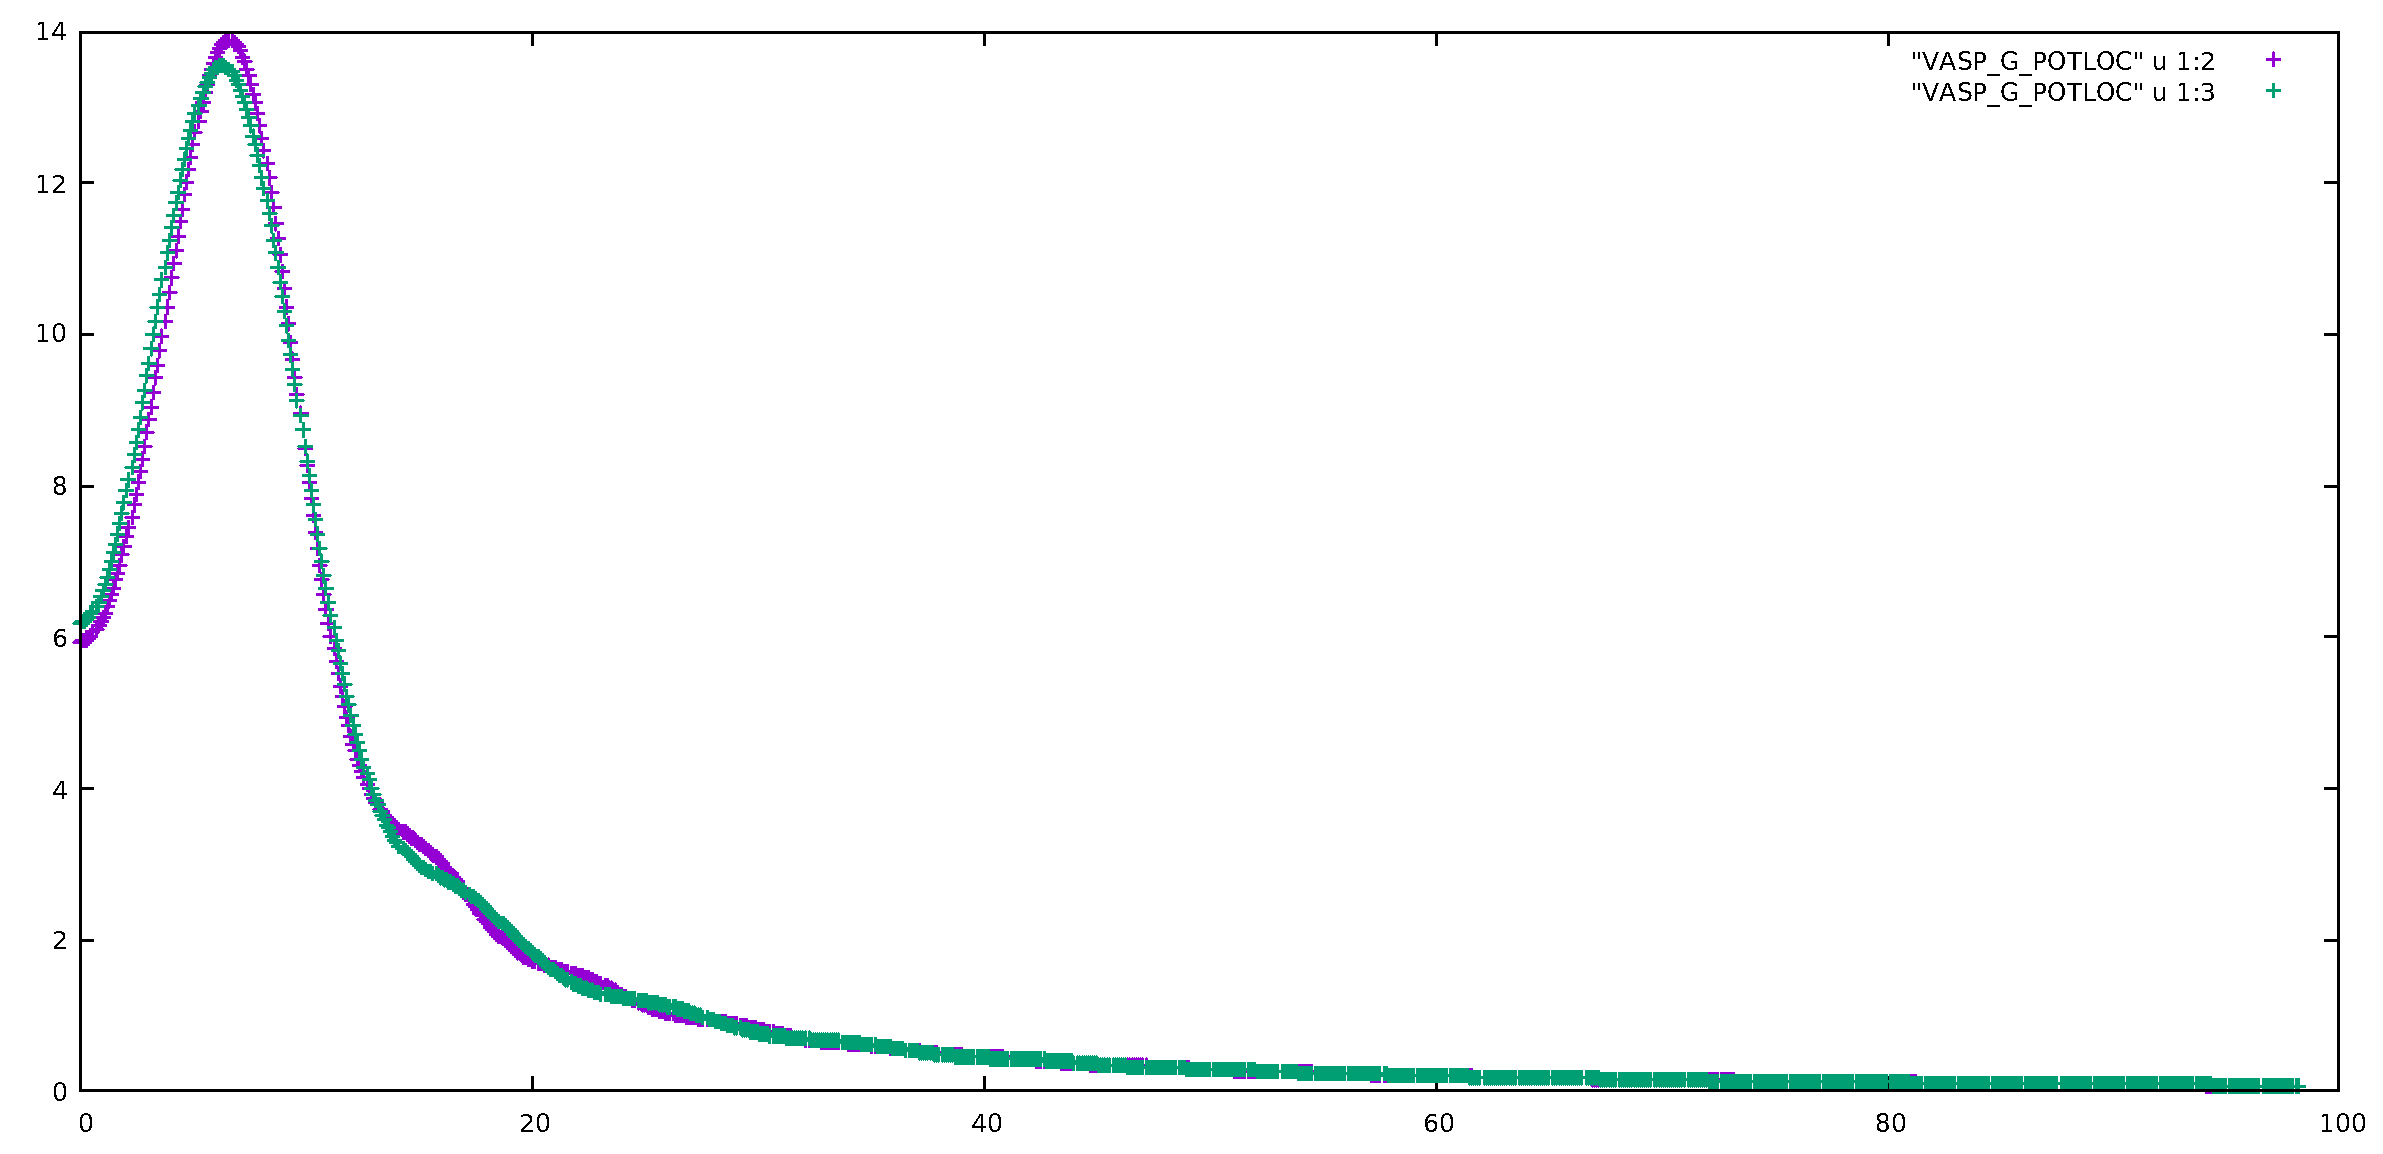
\includegraphics[width=2.3in,height=1.75in,viewport=0 0 1150 650, clip]{Figures/POT_G-dat.pdf}
\label{local-potential}
\end{figure}
\end{minipage}
}

\frame
{
	\frametitle{\rm{VASP}的\rm{POTCAR}}
\begin{minipage}{0.40\textwidth}
\centering
\vspace{-0.05in}
%------------------------------------直-接-插-入-文-件--------------------------------------------------------------------------------------
%\textcolor{red}{\textbf{直接插入文件}}:
\fontsize{2.7pt}{1.2pt}\selectfont{
%\verbatiminput{/home/jiangjun/Documents/Latex_Beamer/Figures/VASP-POTCAR_Si-02-localcorecharge} %为保险:~选用文件名绝对路径
\verbatiminput{Figures/VASP-POTCAR_Si-02-localcorecharge} %为保险:~选用文件名绝对路径
}
\end{minipage}
\begin{minipage}{0.58\textwidth}
{\fontsize{7.2pt}{6.2pt}\selectfont{
	\vskip -5.0in
	\begin{displaymath}
		\begin{aligned}
%			\tilde{V}(q)=&\frac{4\pi}{q}\int\sin(q\cdot r)\tilde{V}(r)\cdot r\mathrm{d}r\\
			\tilde{\rho}_{\mathrm{core}}(q)\cdot q=&4\pi\int_0^{\infty}\sin(q\cdot r)\tilde{\rho}_{\mathrm{core}}(r)\cdot r\mathrm{d}r\\
%			=&\frac{4\pi}{q}\int_0^{\infty}\sin(q\cdot r)V(r)\cdot r\mathrm{d}r
		\end{aligned}
\end{displaymath}
}}
\end{minipage}
}

\frame
{
	\frametitle{\rm{VASP}的\rm{POTCAR}}
\begin{minipage}{0.40\textwidth}
\centering
\centering
\vspace{-0.05in}
%------------------------------------直-接-插-入-文-件--------------------------------------------------------------------------------------
%\textcolor{red}{\textbf{直接插入文件}}:
\fontsize{2.7pt}{1.2pt}\selectfont{
%\verbatiminput{/home/jiangjun/Documents/Latex_Beamer/Figures/VASP-POTCAR_Si-03-pseudo-charge} %为保险:~选用文件名绝对路径
\verbatiminput{Figures/VASP-POTCAR_Si-03-pseudo-charge} %为保险:~选用文件名绝对路径
}
\end{minipage}
\begin{minipage}{0.58\textwidth}
{\fontsize{7.2pt}{6.2pt}\selectfont{
	\vskip -5.0in
	\begin{displaymath}
		\tilde{\rho}(q)=\frac{\tilde{V}(q)}{4\pi}\cdot q^2
\end{displaymath}
}}
\end{minipage}
}

\frame
{
	\frametitle{\rm{VASP}的\rm{POTCAR}}
\begin{minipage}{0.58\textwidth}
\centering
\vspace{-0.10in}
%------------------------------------直-接-插-入-文-件--------------------------------------------------------------------------------------
%\textcolor{red}{\textbf{直接插入文件}}:
\fontsize{2.6pt}{1.2pt}\selectfont{
%\verbatiminput{/home/jiangjun/Documents/Latex_Beamer/Figures/VASP-POTCAR_Si-04-projector-1} %为保险:~选用文件名绝对路径
\verbatiminput{Figures/VASP-POTCAR_Si-04-projector-1} %为保险:~选用文件名绝对路径
}
\end{minipage}
\hfill
\begin{minipage}{0.40\textwidth}
{\fontsize{5.5pt}{4.2pt}\selectfont{
	\begin{displaymath}
		\begin{aligned}
			& G_{\max}^2 \\
			& r_{\max,0}^{\mathrm{pro}}
		\end{aligned}
	\end{displaymath}
	\vskip 10pt
	\begin{displaymath}
		\begin{aligned}
			\hat{T}|\psi_i\rangle=&\left[-\nabla^2-\frac{l(l+1)}2\right]|\psi_i\rangle\\
			D_{ij}^{\mathrm{ion}}=&\langle\psi_i|\hat{T}+V_{\mathrm{eff}}|\psi_j\rangle\\
			-&\langle\tilde{\psi}_i|\hat{T}+\tilde{V}_{\mathrm{eff}}|\tilde{\psi}_j\rangle\\
			-&\int\hat{Q}_{ij}^{00}(r)\tilde{V}(r)\mathrm{d}r
		\end{aligned}
	\end{displaymath}
	\vskip 50pt
	\begin{displaymath}
		\langle\tilde{p}_i|\tilde\phi_j\rangle=\delta_{ij}	
	\end{displaymath}}}
\end{minipage}
}

\frame
{
	\frametitle{\rm{VASP}的\rm{POTCAR}}
\centering
\vspace{-0.15in}
%------------------------------------直-接-插-入-文-件--------------------------------------------------------------------------------------
%\textcolor{red}{\textbf{直接插入文件}}:
\fontsize{2.6pt}{1.2pt}\selectfont{
%\verbatiminput{/home/jiangjun/Documents/Latex_Beamer/Figures/VASP-POTCAR_Si-04-projector-2} %为保险:~选用文件名绝对路径
\verbatiminput{Figures/VASP-POTCAR_Si-04-projector-2} %为保险:~选用文件名绝对路径
}
}

\frame
{
	\frametitle{\rm{VASP}的\rm{POTCAR}}
\centering
\vspace{-0.15in}
%------------------------------------直-接-插-入-文-件--------------------------------------------------------------------------------------
%\textcolor{red}{\textbf{直接插入文件}}:
\fontsize{4.8pt}{4.2pt}\selectfont{
%\verbatiminput{/home/jiangjun/Documents/Latex_Beamer/Figures/VASP-POTCAR_Si-05-augmentcharge} %为保险:~选用文件名绝对路径
\verbatiminput{Figures/VASP-POTCAR_Si-05-augmentcharge} %为保险:~选用文件名绝对路径
}
}

\frame
{
	\frametitle{\rm{VASP}的\rm{POTCAR}}
\begin{minipage}{0.58\textwidth}
\centering
\vspace{-0.10in}
%------------------------------------直-接-插-入-文-件--------------------------------------------------------------------------------------
%\textcolor{red}{\textbf{直接插入文件}}:
\fontsize{3.3pt}{1.9pt}\selectfont{
%\verbatiminput{/home/jiangjun/Documents/Latex_Beamer/Figures/VASP-POTCAR_Si-06-grid} %为保险:~选用文件名绝对路径
\verbatiminput{Figures/VASP-POTCAR_Si-06-grid} %为保险:~选用文件名绝对路径
}
\end{minipage}
\hfill
\begin{minipage}{0.40\textwidth}
{\fontsize{8.2pt}{6.2pt}\selectfont{
	\centering{径向部分的对数布点:}
	\begin{displaymath}
		r(i)=r(1)*10^{(i-1)\cdot\Delta h}
	\end{displaymath}}}
\end{minipage}
}

\frame
{
	\frametitle{\rm{VASP}的\rm{POTCAR}}
\begin{minipage}{0.58\textwidth}
\centering
\vspace{-0.10in}
%------------------------------------直-接-插-入-文-件--------------------------------------------------------------------------------------
%\textcolor{red}{\textbf{直接插入文件}}:
\fontsize{3.3pt}{1.9pt}\selectfont{
%\verbatiminput{/home/jiangjun/Documents/Latex_Beamer/Figures/VASP-POTCAR_Si-07-aepotential} %为保险:~选用文件名绝对路径
\verbatiminput{Figures/VASP-POTCAR_Si-07-aepotential} %为保险:~选用文件名绝对路径
}
\end{minipage}
\hfill
\begin{minipage}{0.40\textwidth}
\begin{figure}[t!]
\centering
\vspace{-0.05in}
\includegraphics[height=2.25in,width=1.5in,viewport=0 0 350 550, angle=-90, clip]{Figures/POTAE-data.eps}
\label{Potential_Function}
\end{figure}
\end{minipage}
}

\frame
{
	\frametitle{\rm{VASP}的\rm{POTCAR}}
\begin{minipage}{0.58\textwidth}
\centering
\vspace{-0.10in}
%------------------------------------直-接-插-入-文-件--------------------------------------------------------------------------------------
%\textcolor{red}{\textbf{直接插入文件}}:
\fontsize{3.3pt}{1.9pt}\selectfont{
%\verbatiminput{/home/jiangjun/Documents/Latex_Beamer/Figures/VASP-POTCAR_Si-08-corecharge} %为保险:~选用文件名绝对路径
\verbatiminput{Figures/VASP-POTCAR_Si-08-corecharge} %为保险:~选用文件名绝对路径
}
\end{minipage}
\hfill
\begin{minipage}{0.40\textwidth}
\begin{figure}[t!]
\centering
\vspace{-0.05in}
\includegraphics[height=2.25in,width=1.5in,viewport=0 0 350 550, angle=-90, clip]{Figures/CORE-data.eps}
\label{core_density_Function}
\end{figure}
\end{minipage}
}

\frame
{
	\frametitle{\rm{VASP}的\rm{POTCAR}}
\centering
\vspace{-0.15in}
%------------------------------------直-接-插-入-文-件--------------------------------------------------------------------------------------
%\textcolor{red}{\textbf{直接插入文件}}:
\fontsize{3.3pt}{1.9pt}\selectfont{
%\verbatiminput{/home/jiangjun/Documents/Latex_Beamer/Figures/VASP-POTCAR_Si-09-kinetic-ene-den} %为保险:~选用文件名绝对路径
\verbatiminput{Figures/VASP-POTCAR_Si-09-kinetic-ene-den} %为保险:~选用文件名绝对路径
}
}

\frame
{
	\frametitle{\rm{VASP}的\rm{POTCAR}}
\begin{minipage}{0.58\textwidth}
\centering
\vspace{-0.10in}
%------------------------------------直-接-插-入-文-件--------------------------------------------------------------------------------------
%\textcolor{red}{\textbf{直接插入文件}}:
\fontsize{3.3pt}{1.9pt}\selectfont{
%\verbatiminput{/home/jiangjun/Documents/Latex_Beamer/Figures/VASP-POTCAR_Si-10-pspotential} %为保险:~选用文件名绝对路径
\verbatiminput{Figures/VASP-POTCAR_Si-10-pspotential} %为保险:~选用文件名绝对路径
}
\end{minipage}
\hfill
\begin{minipage}{0.40\textwidth}
\begin{figure}[t!]
\centering
\vspace{-0.05in}
\includegraphics[height=2.25in,width=1.5in,viewport=0 0 350 550, angle=-90, clip]{Figures/POTPSC-data.eps}
\label{Pseudopotential-core_Function}
\end{figure}
\end{minipage}
}

\frame
{
	\frametitle{\rm{VASP}的\rm{POTCAR}}
\begin{minipage}{0.58\textwidth}
\centering
\vspace{-0.10in}
%------------------------------------直-接-插-入-文-件--------------------------------------------------------------------------------------
%\textcolor{red}{\textbf{直接插入文件}}:
\fontsize{3.3pt}{1.9pt}\selectfont{
%\verbatiminput{/home/jiangjun/Documents/Latex_Beamer/Figures/VASP-POTCAR_Si-11-pscoreden} %为保险:~选用文件名绝对路径
\verbatiminput{Figures/VASP-POTCAR_Si-11-pscoreden} %为保险:~选用文件名绝对路径
}
\end{minipage}
\hfill
\begin{minipage}{0.40\textwidth}
\begin{figure}[t!]
\centering
\vspace{-0.05in}
\includegraphics[height=2.25in,width=1.5in,viewport=0 0 350 550, angle=-90, clip]{Figures/PCORE-data.eps}
\label{psedudocore_density_Function}
\end{figure}
\end{minipage}
}

\frame
{
	\frametitle{\rm{VASP}的\rm{POTCAR}}
\begin{minipage}{0.58\textwidth}
\centering
\vspace{-0.10in}
%------------------------------------直-接-插-入-文-件--------------------------------------------------------------------------------------
%\textcolor{red}{\textbf{直接插入文件}}:
\fontsize{3.3pt}{1.9pt}\selectfont{
%\verbatiminput{/home/jiangjun/Documents/Latex_Beamer/Figures/VASP-POTCAR_Si-12-pswav-1} %为保险:~选用文件名绝对路径
\verbatiminput{Figures/VASP-POTCAR_Si-12-pswav-1} %为保险:~选用文件名绝对路径
}
\end{minipage}
\hfill
\begin{minipage}{0.40\textwidth}
\begin{figure}[t!]
\centering
\vspace{-0.05in}
\includegraphics[height=2.25in,width=1.4in,viewport=0 0 350 550, angle=-90, clip]{Figures/WAE-data.eps}
\label{Wave-AE_Function}
\end{figure}
\end{minipage}
}

\frame
{
	\frametitle{\rm{VASP}的\rm{POTCAR}}
\begin{minipage}{0.58\textwidth}
\centering
\vspace{-0.10in}
%------------------------------------直-接-插-入-文-件--------------------------------------------------------------------------------------
%\textcolor{red}{\textbf{直接插入文件}}:
\fontsize{3.3pt}{1.9pt}\selectfont{
%\verbatiminput{/home/jiangjun/Documents/Latex_Beamer/Figures/VASP-POTCAR_Si-12-aewav-1} %为保险:~选用文件名绝对路径
\verbatiminput{Figures/VASP-POTCAR_Si-12-aewav-1} %为保险:~选用文件名绝对路径
}
\end{minipage}
\hfill
\begin{minipage}{0.40\textwidth}
\begin{figure}[t!]
\centering
\vspace{-0.05in}
\includegraphics[height=2.25in,width=1.4in,viewport=0 0 350 550, angle=-90, clip]{Figures/WPS-data.eps}
\label{Wave-PS_Function}
\end{figure}
\end{minipage}
}

\frame
{
	\frametitle{\rm{VASP}的\rm{POTCAR}}
\centering
\vspace{-0.15in}
%------------------------------------直-接-插-入-文-件--------------------------------------------------------------------------------------
%\textcolor{red}{\textbf{直接插入文件}}:
\fontsize{3.3pt}{1.9pt}\selectfont{
%\verbatiminput{/home/jiangjun/Documents/Latex_Beamer/Figures/VASP-POTCAR_Si-12-pswav-2} %为保险:~选用文件名绝对路径
\verbatiminput{Figures/VASP-POTCAR_Si-12-pswav-2} %为保险:~选用文件名绝对路径
}
}

\frame
{
	\frametitle{\rm{VASP}的\rm{POTCAR}}
\centering
\vspace{-0.15in}
%------------------------------------直-接-插-入-文-件--------------------------------------------------------------------------------------
%\textcolor{red}{\textbf{直接插入文件}}:
\fontsize{3.3pt}{1.9pt}\selectfont{
%\verbatiminput{/home/jiangjun/Documents/Latex_Beamer/Figures/VASP-POTCAR_Si-12-aewav-2} %为保险:~选用文件名绝对路径
\verbatiminput{Figures/VASP-POTCAR_Si-12-aewav-2} %为保险:~选用文件名绝对路径
}
}

\frame
{
	\frametitle{\rm{VASP}的\rm{POTCAR}}
\centering
\vspace{-0.15in}
%------------------------------------直-接-插-入-文-件--------------------------------------------------------------------------------------
%\textcolor{red}{\textbf{直接插入文件}}:
\fontsize{3.3pt}{1.9pt}\selectfont{
%\verbatiminput{/home/jiangjun/Documents/Latex_Beamer/Figures/VASP-POTCAR_Si-12-pswav-3} %为保险:~选用文件名绝对路径
\verbatiminput{Figures/VASP-POTCAR_Si-12-pswav-3} %为保险:~选用文件名绝对路径
}
}

\frame
{
	\frametitle{\rm{VASP}的\rm{POTCAR}}
\centering
\vspace{-0.15in}
%------------------------------------直-接-插-入-文-件--------------------------------------------------------------------------------------
%\textcolor{red}{\textbf{直接插入文件}}:
\fontsize{3.3pt}{1.9pt}\selectfont{
%\verbatiminput{/home/jiangjun/Documents/Latex_Beamer/Figures/VASP-POTCAR_Si-12-aewav-3} %为保险:~选用文件名绝对路径
\verbatiminput{Figures/VASP-POTCAR_Si-12-aewav-3} %为保险:~选用文件名绝对路径
}
}

\frame
{
	\frametitle{\rm{VASP}的\rm{POTCAR}}
\centering
\vspace{-0.15in}
%------------------------------------直-接-插-入-文-件--------------------------------------------------------------------------------------
%\textcolor{red}{\textbf{直接插入文件}}:
\fontsize{3.3pt}{1.9pt}\selectfont{
%\verbatiminput{/home/jiangjun/Documents/Latex_Beamer/Figures/VASP-POTCAR_Si-12-pswav-4} %为保险:~选用文件名绝对路径
\verbatiminput{Figures/VASP-POTCAR_Si-12-pswav-4} %为保险:~选用文件名绝对路径
}
}

\frame
{
	\frametitle{\rm{VASP}的\rm{POTCAR}}
\centering
\vspace{-0.15in}
%------------------------------------直-接-插-入-文-件--------------------------------------------------------------------------------------
%\textcolor{red}{\textbf{直接插入文件}}:
\fontsize{3.3pt}{1.9pt}\selectfont{
%\verbatiminput{/home/jiangjun/Documents/Latex_Beamer/Figures/VASP-POTCAR_Si-12-aewav-4} %为保险:~选用文件名绝对路径
\verbatiminput{Figures/VASP-POTCAR_Si-12-aewav-4} %为保险:~选用文件名绝对路径
}
}

